\subsection{Kryptographischer Hintergrund}
\label{sec:crypto}

Eine kryptographische Hashfunktion, auch \glqq Message Digest\grqq -Funktion genannt ist
eine Familie von Hashing Algorithmen
, die eine Nachricht $m$ auf einen \glqq Digest\grqq $\ h(m)$ reduzieren.
Die Idee ist also
eine Nachricht durch Hashing kompakt zu repräsentieren, was bspw.
für Signaturen
von langen Texten Anwendung findet~\cite{menezes2018} und \
da beim Hashing  das Urbild der Funktion in der Mächtigkeit die Ergebnismenge deutlich
übersteigt, ist es allerdings möglich sogenannte Kollisionen zu finden, also ein
$m_k \ne m$ mit $h(m) = h(m_k)$.
Für kryptographische Hashfunktionen wurden
entsprechend Eigenschaften festgelegt, die aus einer Sicherheitsperspektive
erstrebenswert sind:\cite{kryptografischeHashfunktion}

\begin{itemize}
      \item [(1)] $\forall m:  H(m)$ ist einfach zu berechnen.
      \item [(2)] \textbf{Urbildresistenz:} Für ein gegebenes $h = H(m)$ ist das Bestimmen des
            Wertes $m$ mit $m = H^{-1}(h)$ nicht effizient möglich, d.h.\ es ist nicht effizient
            möglich mittels $H(m)$ auf $m$ zu schließen.
      \item [(3)] \textbf{schwache Kollisionsresistenz:} Es ist nicht effizient möglich zu einem
            gegebenem $m$ ein $m'$ zu finden, sodass $H(m) = H(m')$.
      \item [(4)] \textbf{starke Kollisionsresistenz:} Es ist nicht effizient möglich ein
            beliebiges Paar $(m, m')$ zu finden, sodass $H(m) = H(m')$.
\end{itemize}

MD2 Hashing besteht aus 3 Schritten. Zuerst wird die Nachricht auf ein
Vielfaches von 16 Byte ergänzt. Anschließend wird eine Prüfsumme berechnet und 
an das Ende der Nachricht angehängt. Zum Schluss wird die Nachricht in 18 
Durchläufen komprimiert oder gehasht. 
Wir werden auf jeden dieser Schritte im Detail eingehen. 

\subsection{PKCS\#7 Padding: Implementierung und Optimierung}

In der kryptographischen Welt ist das Padding von Nachrichten eine weit verbreitete
Technik, um die Größe der zu verarbeitenden Daten auf ein Vielfaches der Blocklänge
zu bringen.
Ein gängiges Verfahren dafür ist das PKCS\#7 Padding, das hier genauer
erörtert wird.
Es handelt sich um ein standardisiertes Verfahren, das in RFC 2315
ausführlich beschrieben wird~\cite{rfc2315}.
\\
Die grundlegende Idee des PKCS\#7 Paddings besteht darin, den fehlenden Platz in
einem Block mit einer Sequenz von Bytes zu füllen, deren Wert der Länge der
Sequenz entspricht.
Bei einer Blocklänge von 16 Bytes kann also jeder Block,
unabhängig von seiner ursprünglichen Größe, auf die erforderliche Länge gebracht werden.
\\
Eine Optimierungsstufe kann durch den Einsatz von SIMD-Instruktionen erreicht
werden, wie in der Funktion \texttt{padding\_opt\_V0} gezeigt.
Durch die Verwendung
der SIMD-Instruktion \texttt{\_mm\_storeu\_si128} können mehrere Bytes gleichzeitig
geschrieben werden, was zu einer deutlich verbesserten Leistung führt.
\\
Insgesamt ermöglichen diese Optimierungen eine effizientere Anwendung des PKCS\#7
Paddings, was in vielen kryptographischen Kontexten von großem Nutzen sein kann.

\subsection{Berechnung der Prüfsumme}

Die Berechnung der Prüfsumme und des Hashwerts sind zentrale Bestandteile des
MD2-Algorithmus. Ohne dem Prüfsummen-Byte ist der MD2 unsicher \cite{rogier1997}.
In diesem Abschnitt wird die genaue Funktionsweise dieser
Berechnungen erläutert und der Einsatz der Substitutionsbox (S-Box) in diesen
Prozessen verdeutlicht.
Die S-Box, die in diesen Berechnungen verwendet wird, ist ein wesentliches
Element.
Es handelt sich um ein festes, vordefiniertes Array von 256 Werten,
das für die Substitution der Eingabewerte verwendet wird.
Die Werte in der S-Box
sind so gewählt, dass sie den kryptographischen Sicherheitsanforderungen genügen
und das Ausgabebild stark verändern, selbst wenn nur kleine Änderungen an der
Eingabe vorgenommen werden (Diffusion).
Die Prüfsumme wird erstellt, indem eine Checksummen-Funktion auf die Nachricht
angewendet wird, wobei jedes Byte der Nachricht in 16 Byte Blöcken verarbeitet wird.
Das aktuelle Byte des Blocks nennen wir von nun $b_i$ und das 16 Byte Array der
Checksumme $s$.
Ein laufender Totalisator $l$ beginnt am Anfang der Funktion zunächst bei Null $c = 0$.
Anschließend wird der  Index des nächsten Wertes aus der Substitutionsbox mit
$t = b_i \oplus l$ berechnet.
Die Prüfsumme wird an dem Index $i$ dann auf $s_i \oplus t$ gesetzt und letztlich
der Totalisator mit $l = s_i$ aktualisiert.
\\
Die S-Box oder S-Tabelle wird in RFC 1319 \cite{rfc1319} beschrieben wie folgt:
\begin{quote}
    This step uses a 256-byte "random" permutation constructed from the digits of $\pi$.      
\end{quote}
Wirft man allerdings einen Blick auf die S-Box ist es schwer den Zusammenhang 
zwischen den Werten in der Tabelle und $\pi$ zu erkennen. 
Ron Rivest klärte dies in einer E-Mail an einen Forennutzer auf. Zur 
Generierung der S-Box wird $\pi$ als Psuedozufallsgenerator verwendet und mittels 
einer modifizierten Form des Durstenfeld-Shuffles wird eine gleichmäßige Verteilung der
Zufallszahlen in der S-Box ermöglicht.\cite{crypto_stackexchange_18444}

\begin{figure}[h]
      \centering
      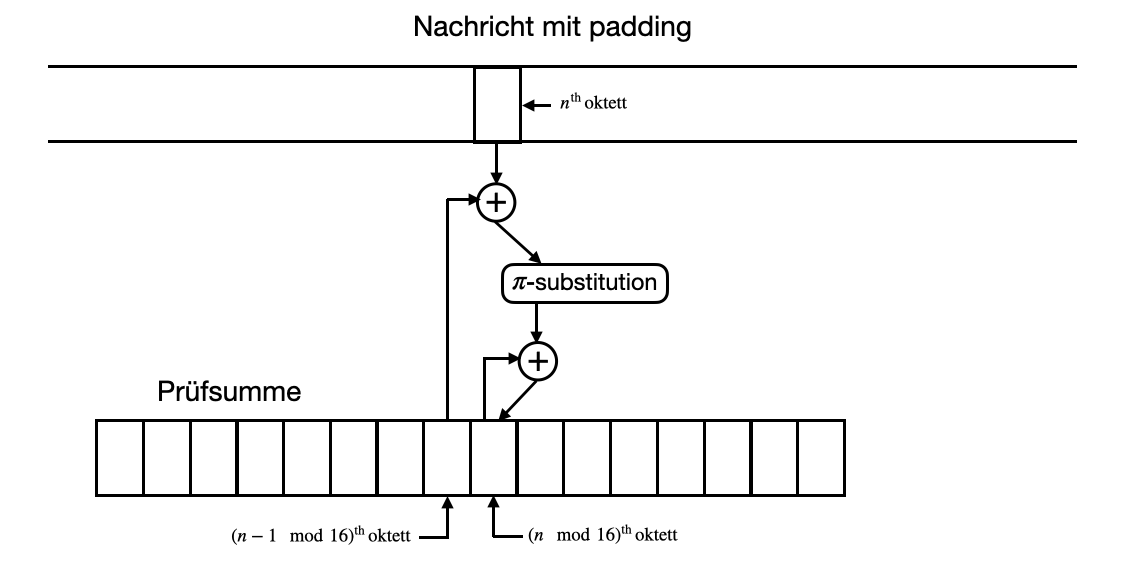
\includegraphics[scale=0.6]{pics/md2diagramchecksum.jpg}
      \caption{Darstellung zur Berechnung der Prüfsumme von MD2\cite{jain2009}}
\end{figure}

Diese genaue Berechnungsmethode, kombiniert mit der Verwendung der S-Box,
trägt zur Sicherheit und Unveränderlichkeit der MD2-Hashfunktion bei.

\subsection{Kompressionsfunktion}


Bei der Kompressionsfunktion handelt es sich um einen iterativen Prozess, bei dem 
mehrere Berechnungsschritte ausgeführt werden, die schließlich zu einem 128-Bit-Hashwert 
führen. Zunächst wird der zu verarbeitende Nachrichtenpuffer in Blöcke von 16 
Bytes aufgeteilt und diese sequenziell verarbeitet. Jeder Block wird in das 
interne Speicher-Array kopiert, das insgesamt 48 Bytes aufnehmen kann und in drei 
Segmente von je 16 Bytes unterteilt ist. Es ist hervorzuheben, dass die ersten 
beiden Segmente vor der Verarbeitung jedes Blocks bereits Daten enthalten können, 
die aus vorherigen Durchläufen stammen. Anschließend wird eine XOR-Operation 
(exklusives Oder) auf den ersten und zweiten Segment des internen Arrays angewendet 
und das Ergebnis in das dritte Segment gespeichert. Das Ergebnis dieser Operation 
fügt eine weitere Ebene der Durchmischung der Daten hinzu und erhöht so die Diffusion 
der Hash-Funktion. Darauf folgen 18 Runden von Substitution und Permutation, die 
auf das gesamte interne Array angewendet werden. In jeder Runde wird jedes Byte 
des internen Arrays durch einen Wert aus der S-Box ersetzt, wobei der Ersatzwert 
durch eine XOR-Operation mit einem temporären Wert bestimmt wird. Nach jeder 
Substitution wird der temporäre Wert aktualisiert, um den nächsten S-Box-Index zu 
bestimmen. Obwohl diese Methode effektiv ist, bietet sie wenig Spielraum für 
Optimierungen. Dies liegt vor allem an der Natur des MD2-Algorithmus, der keine 
Parallelität in seinen Operationen zulässt. Jeder Schritt in der Berechnung ist 
voneinander abhängig und muss in einer strengen Reihenfolge ausgeführt werden. 
Daher sind die Möglichkeiten für Verbesserungen in Bezug auf die Geschwindigkeit 
und Effizienz des Algorithmus begrenzt.

\begin{figure}[h]
      \centering
      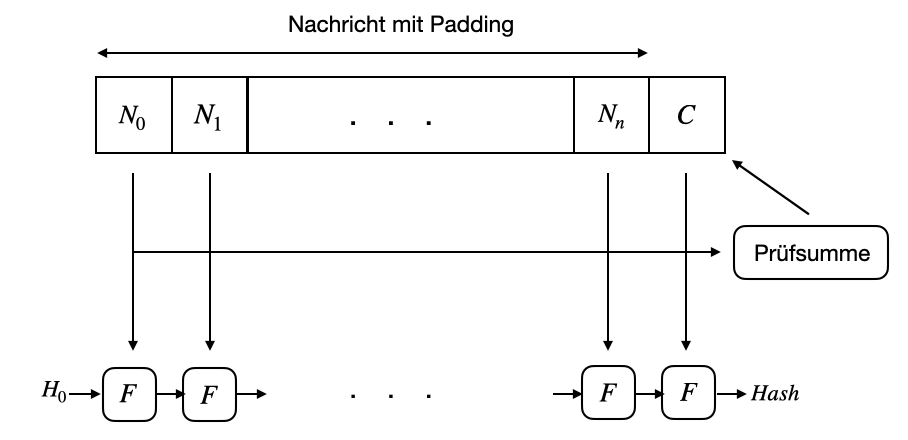
\includegraphics[scale=0.6]{pics/md2.001.jpeg}
      \caption{Berechnung des Hashwertes. $H_0$ beträgt bei MD2 0. 
      Die Darstellung orientiert sich an \cite{knudsen2005}}
\end{figure}


\subsection{Sicherheitsanalyse}

In diesem Abschnitt setzten wir uns konkret mit der kryptographischen Sicherheit 
von MD2 Hashing aus. Hier betrachten wir neben Anwendungsmöglichkeiten auch 
Sicherheitsrisiken und Angriffsvektoren.

\subsubsection{Anwendungsbereiche}
Der MD2-Algorithmus besitzt in der Implementierung eine geringe Komplexität 
und ist zudem schnell berechenbar. Bevor man sicherere Algorithmen entwickelte,
gab es viele Anwedungen für MD2, z.B\@.
\begin{itemize}
      \item \textbf{Überprüfung von Benutzerpasswörtern}
            \\
            Der MD2-Algorithmus kann für die Passwortüberprüfung bei der Benutzeranmeldung
            verwendet werden, indem er vom Klartextabgleich zum Geheimtextabgleich übergeht.
            Hierbei kommt oft auch sog. \glqq Salting \grqq zum Einsatz. Diese Methode 
            wird im Abschnitt \ref{lo:sec_sol} näher behandelt.
      \item \textbf{Überprüfung von Dateiintegrität}
            \\
            Lädt man eine Datei im Internet herunter, kann man oftmals den MD2-Wert 
            der Datei auf der Webseite finden.
            Nachdem der Download abgeschlossen ist, kann der MD2-Wert der heruntergeladenen Datei
            berechnet und mit dem MD2-Wert der Quelle verglichen werden.
            Wenn sie übereinstimmen, ist die Datei vollständig und wurde nicht manipuliert.
            Dadurch kann man die Echtheit der Datei validieren. Natürlich muss 
            hierfür der Hashwert auf der Webseite vertrauenswürdig sein.
     % Leaving this out as this is essentially the same content as the previous point.
      %\item  \textbf{Erkennung von Urheberrechtsverletzung}
      %      \\
      %      Wenn ein Artikel, ein Video oder eine Audiodatei erstellt wird, 
      %      hat sie einen eindeutigen MD2-Wert.
      %      Wenn später eine überarbeitete Version herauskommt, werden die MD2-Werte trotz igleichem
      %      Dateinamen als unterschiedlich eingestuft.
      %      Das Urheberrecht kann anhand des Tags und des MD2-Werts der Datei überprüft werden.
     
\end{itemize}

\subsubsection{Sicherheitslücken}
Von der Verwendung von MD2 Hashing im Internet wird seit 2011 offiziell abgeraten,
doch schon seit 2004 wurde MD2 weitesgehend von MD5 abgelöst. \cite{rfc6149}
Grund dafür sind verschiedene Sicherheitslücken im Algoritmus,
die einen Angriff ermöglichen.
\\
Die Länge des Hashwerts von MD2 beträgt nur 128 bit  bzw $2^{65}$. 
Wegen des Geburtstagsparadoxons sind nur ca. $2^{65/2} = 2^{64}$ Versuche notwendig 
um mit einer Wahrscheinlichkeit von mehr als 50\% eine Kollision zu finden.
Diese relativ kleine Anzahl an Versuchen ist heutzutage effizient leistbar. 
Folglich sind auch komplexere Kollisionsangriffe auf MD2 nicht nötig, da die rohe 
Rechenleistung von heutigen Supercomputern genügt, um ein Kollisionspaar zu 
finden.\cite{kryptografischeHashfunktion}
\\
Das größere Sicherheitsproblem ist die schwache Urbildresistenz von MD2. Der
französische Informatiker Fr{\'e}d{\'e}ric Muller fand 2004 erstmals eine Möglichkeit 
das Urblid eines Hashwertes in besserer Laufzeit als Bruteforce zu ermitteln.
Seine Methode beruht darauf zuerst verschiedene Urbilder der Kompressionsfunktion zu finden, 
was durch den Initialisierungsvektor $0$ möglich ist und anschließend 
die Prüfsummen abzugleichen um ein korrektes Urbild zu ermitteln. 
Die Zeitkomplexität dieser Methode beträgt ca. $2^{104}$ \cite{knudsen2005}, 
was unter den von NIST vorgeschriebenen 128-bit an Sicherheit liegt.\cite{barker2020}
\\
Diese schwache Urbildresistenz wird in sogenannten Rainbow Tables zu 
Nutze gemacht.\cite{oechslin2003}
Diese berechnen die Hashwerte für verschiedenste Passwortkombinationen vor und 
speichern sie in einer Kette, die zwischen Hashwerten und Passwörtern alterniert. 
Dafür muss natürlich die Hashfunktion bekannt sein und auch eine Reduktionsfunktion,
auf deren Details wir im Rahmen dieser Ausarbeitung nicht weiter eingehen,
auf die Hashwerte angewendet werden um wieder Klartexte zu erhalten. 
Mithilfe dieser vorberechneten Werte, erlaubt man sich einen Zeit-Speicher-Ausgleich.

\subsubsection{Sicherheitsmaßnahmen}

%left out due to space limitation
%Diese Schwachstellen haben verschiedene Verwenbarkeiten. Dies sind nur ein Paar
%Konsequenzen die aus einem Angriff entstehen könnten:

%\begin{itemize}
      %\item  \textbf{verfälschte Anmeldeauthentifizierung}
            %\\
            %Wenn die Authentifizierung ein Vergleich von Hashwerten ist, 
            %kann der Angreifer sich mittels einer Hashkollision anmelden.
            %Hierbei muss er nicht einmal das exakte Passwort des Nutzers finden.
      %\item  \textbf{verfälschte digitale Signaturen}
            %\\
            %Wenn Alice (A) und Bob (B) miteinander kommunizieren, fängt ein
            %Man-in-the-Middle-Angreifer (M) die von A an B gesendete Nachricht ab.
            %Da der MD2-Algorithmus öffentlich ist, kann M den ursprünglichen Hashwert der
            %Nachricht berechnen und dann eine neue Nachricht mit demselben Hashwert erzeugen
            %und an B weiterleiten
            %Bisher kann M die gesamte Kommunikation zwischen A und B überwachen und manipulieren,
            %was für A und B schwierig zu erkennen ist.
            %Somit sind Datenintegrität und Authentizität sind gebrochen.
%\end{itemize}
%
%\subsubsection{Verbesserung der kryptografischen Sicherheit}
\label{lo:sec_sol}
\begin{itemize}
      \item \textbf{Salz zur Hashfunktion hinzufügen}
            \\
            Die Hashfunktion wird zu $hash(salt + str)$. \cite{kryptografischeHashfunktion}
            Da der Salt nicht öffentlich verfügbar ist, wird es für einen Angreifer schwieriger,
            Zeichenketten mit identischen Hashwerten zu konstruieren.
            Hierbei wird vor dem 
            Hashing das Klartextwort um einen zufälligen ASCII
            string ergänzt. Dies führt durch Diffusion zu wesentlich anderen Hashwerten als sonst 
            und schützt das System vor Angriffen durch Rainbow Tables. 
            Zudem müsste ein Angreifen dann neben den Passwörtern auch alle möglichen Salts 
            in einem Brute-Force Angriff beachten.
      \item \textbf{Hash-Kollisionen vermeiden}
            \\
            Die Verwendung von Rehash oder geschlossenem Hashing mit offener Adressierung
            sind wirksame Verfahren zur Vermeidung von Hash-Kollisionen.\cite{hashtabelle}
            Jedoch führen sie zu einem Anstieg der Rechenzeit bzw. des Speicherplatzes.
      \item \textbf{Modernere Hashfunktionen verwenden}
            \\
            Es wird von NIST nicht empfohlen, MD2, MD4, MD5, SHA-1, RIPEMD-Algorithmen zu verwenden,
            um sensible Informationen wie Benutzerpasswörter zu
            sichern. \cite{barker2020}
            SHA-512, SHA-3 oder andere fortschrittlichere Hashfunktionen 
            wären bessere Optionen.
\end{itemize}